%! Author = sutingchen
%! Date = 2023/10/20

\titledquestion{Left Child Right Sibling}

\begin{parts}
    \part[1] For every ordered tree, there is a unique representation of Left-child right-sibling format.

    \begin{oneparcheckboxes}
        \CorrectChoice True
        \choice False
    \end{oneparcheckboxes}

    \part[1] Pre-order traversal of the original tree is identical to the pre-order traversal of the Knuth transform.

    \begin{oneparcheckboxes}
        \CorrectChoice True
        \choice False
    \end{oneparcheckboxes}

    \part[1] Post-order traversal of the original tree is identical to the post-order traversal of the Knuth transform.

    \begin{oneparcheckboxes}
        \choice True
        \CorrectChoice False
    \end{oneparcheckboxes}


    \part[7] Transform the tree below with root \textbf{1} (in LCRS format) to N-ary format.

    \begin{figure}[h]
        \centering
        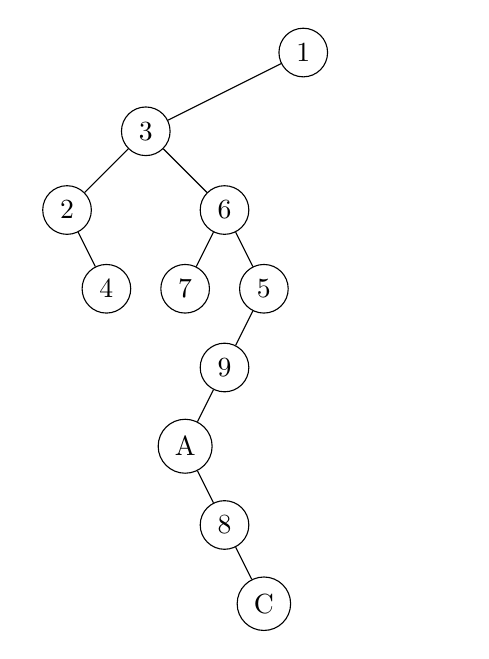
\begin{tikzpicture}[level distance=1cm,
                level 1/.style={sibling distance=4cm},
                level 2/.style={sibling distance=2cm},
                level 3/.style={sibling distance=1cm},
                every node/.style = {draw, circle}]
            \node {1}
            child { node {3}
                    child { node {2}
                            child { edge from parent[draw=none] }
                            child { node {4} }
                        }
                    child { node {6}
                            child { node {7} }
                            child { node {5}
                                    child { node {9}
                                            child { node {A}
                                                    child { edge from parent[draw=none] }
                                                    child { node {8}
                                                            child { edge from parent[draw=none] }
                                                            child { node {C} }
                                                        }
                                                }
                                            child { edge from parent[draw=none] }
                                        }
                                    child { edge from parent[draw=none] }
                                }
                        }
                }
            child { edge from parent[draw=none] };
        \end{tikzpicture}

        \label{fig:LCRS_question}
    \end{figure}

    \begin{solution}
        %\vspace{10em}
        \begin{center}
            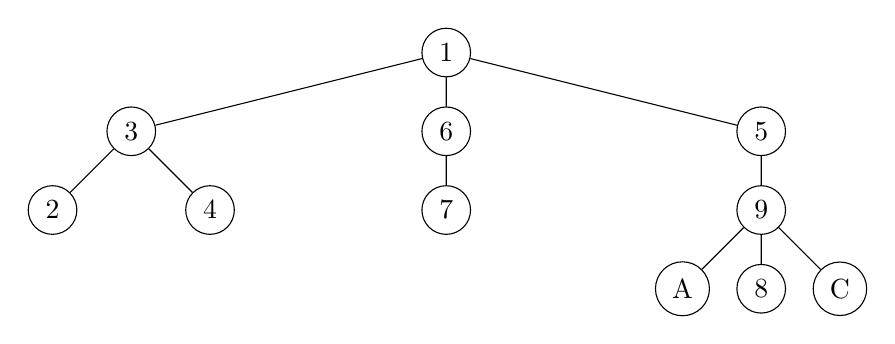
\begin{tikzpicture}[level distance=1cm,
                    level 1/.style={sibling distance=4cm},
                    level 2/.style={sibling distance=2cm},
                    level 3/.style={sibling distance=1cm},
                    every node/.style = {draw, circle}]
                \node {1}
                child { node {3}
                        child { node {2} }
                        child { node {4} }
                    }
                child { node {6}
                        child { node {7} }
                    }
                child { node {5}
                        child { node {9}
                                child { node {A} }
                                child { node {8} }
                                child { node {C} }
                            }
                    };
            \end{tikzpicture}
        \end{center}
    \end{solution}

\end{parts}
